\documentclass[10pt]{beamer}
\usetheme{Madrid}
\setbeamercovered{dynamic}
\setbeamertemplate{navigation symbols}{}

\usepackage[T1]{fontenc}
\usefonttheme{professionalfonts}
\usepackage[sfmath,slantedGreeks]{kpfonts}
\usepackage[utf8]{inputenc}

\usepackage[hyperref,backend=biber,maxbibnames=4,firstinits=true]{biblatex}
\usepackage{graphicx,siunitx}
\usepackage[font=scriptsize,labelformat=empty]{caption}

\DeclareSIUnit\parsec{pc}
\DeclareSIUnit\clight{\text{\ensuremath{c}}}
\sisetup{per-mode=symbol,
  inter-unit-separator={}\cdot{},
  exponent-product=\cdot,
  output-product=\cdot,
  separate-uncertainty=true
}

\addbibresource{bibliography.bib}
\newcommand{\arxiv}[1]{{\usebeamercolor[fg]{bibliography entry note}
    \href{http://arxiv.org/abs/#1}{arXiv: \texttt{#1}}}}
\newcommand{\doi}[1]{{\usebeamercolor[fg]{bibliography entry note}
    \href{http://dx.doi.org/#1}{\textsc{doi}: \texttt{#1}}}}

\DeclareMathOperator{\e}{\mathrm{e}}
\DeclareMathOperator{\uimm}{\mathrm{i}} % unità immaginaria
\renewcommand{\phi}{\varphi}

\newcommand{\advice}{
\includegraphics[height=0.8em]{figures/light-bulb}}
\newcommand{\warning}{
\includegraphics[height=0.6em]{figures/Warning-icon}}

\title[Estimating orbital period of exoplanets in microlensing
events]{Estimating orbital period of exoplanets \\ in microlensing events}

\author{Mosè Giordano}
\date{25 September 2014}
\institute[UniSalento and INFN Lecce]{Università del Salento and INFN Lecce}
\titlegraphic{
\includegraphics[width=20mm]{figures/logo-unisalento}}

% Customise the caption: do not insert the caption name, nor the number, just
% insert a smaller caption text.
\setbeamertemplate{caption}{\scriptsize\insertcaption}

%% Personalizzo modello prima pagina
\setbeamercolor*{institute}{parent=palette primary}
\defbeamertemplate*{title page}{customized}[1][]
{
  \vbox{}
  \vfill
  \centering
  % Nome Università
  \mbox{\begin{beamercolorbox}[rounded=true,shadow=true,ht=2.5ex,
      wd=0.7\paperwidth,sep=3pt,center]{institute}%
      \large\scshape\insertinstitute\par%
    \end{beamercolorbox}}
  % Logo
  \vskip0.5em
  {\usebeamercolor[fg]{titlegraphic}
    
\includegraphics[width=20mm]{figures/logo-unisalento}\quad
    
\includegraphics[width=50mm]{figures/dipartimento}\quad
    
\includegraphics[width=20mm]{figures/infn}\par}
  \vskip0.25em%
  % Titolo
  \begin{beamercolorbox}[sep=8pt,center,#1]{title}
    \usebeamerfont{title}\inserttitle\par%
    % Decommenta se c'è un sottotitolo
    \ifx\insertsubtitle\@empty%
    \else%
    \vskip0.25em%
    {\usebeamerfont{subtitle}\usebeamercolor[fg]{subtitle}\insertsubtitle\par}%
    \fi%
  \end{beamercolorbox}%
  \vskip1em\par
  \begin{center}
    \emph{Mosè Giordano}        \\[4ex]
    Summer Course on Exoplanets \\[2ex]
    La Palma, Canary Islands    \\[2ex]
    \insertdate
  \end{center}
  \vfill
}

\makeatletter
\defbeamertemplate*{footline}{customized}
{
  \leavevmode%
  \hbox{%
  \begin{beamercolorbox}[wd=.3\paperwidth,ht=2.25ex,dp=1ex,center]{author in head/foot}%
    \usebeamerfont{author in head/foot}\insertshortauthor\expandafter\beamer@ifempty\expandafter{\beamer@shortinstitute}{}{~~(\insertshortinstitute)}
  \end{beamercolorbox}%
  \begin{beamercolorbox}[wd=.4\paperwidth,ht=2.25ex,dp=1ex,center]{title in head/foot}%
    \usebeamerfont{title in head/foot}\insertshorttitle
  \end{beamercolorbox}%
  \begin{beamercolorbox}[wd=.3\paperwidth,ht=2.25ex,dp=1ex,right]{date in head/foot}%
    \usebeamerfont{date in head/foot}\insertshortdate{}\hspace*{2em}
    \insertframenumber{} / \inserttotalframenumber\hspace*{2ex} 
  \end{beamercolorbox}}%
  \vskip0pt%
}
\makeatother

%%% Beamer colors %%%%%%%%%%%%%%%%%%%%%%%%%%%%%%%%%%%%%%%%%%%%%%%%%%%%%%
% Some tango colors
% butter (yellowish)
\definecolor{tabutter}{rgb}{0.98824, 0.91373, 0.30980}		% #fce94f

% orange
\definecolor{taorange}{rgb}{0.98824, 0.68627, 0.24314}		% #fcaf3e
\definecolor{ta2orange}{rgb}{0.96078, 0.47451, 0}		% #f57900

% Custom colors
\definecolor{mm3orange}{rgb}{0.90784, 0.36078, 0}
\definecolor{mmskyblue}{rgb}{0.34706, 0.56078, 0.81176}
\definecolor{mm2skyblue}{rgb}{0.10392, 0.39608, 0.64314}
\definecolor{mm3skyblue}{rgb}{0.02549, 0.29020, 0.52941}
\definecolor{mmLightSteelBlue}{rgb}{.5, .77, .87}

\setbeamercolor{normal text}{fg=black,bg=white}
\setbeamercolor{alerted text}{fg=mm3orange}
\setbeamercolor*{example text}{fg=lightgray,bg=black}

\setbeamercolor{structure}{fg=mm2skyblue}

% \setbeamercolor{title in head/foot}{fg=white, bg=mmskyblue}
% \setbeamercolor{author in head/foot}{fg=white, bg=mm3skyblue}

\setbeamertemplate{itemize items}[circle]

\setbeamercolor{headline}{fg=tabutter,bg=mm3skyblue}
\setbeamercolor{footline}{fg=tabutter, bg=mm3skyblue}
\setbeamercolor{separation line}{bg=ta2orange}
\setbeamercolor{framesubtitle}{fg=white, bg=ta2gray}
%%%%%%%%%%%%%%%%%%%%%%%%%%%%%%%%%%%%%%%%%%%%%%%%%%%%%%%%%%%%%%%%%%%%%%%%

\begin{document}
\begin{frame}[plain]
  \maketitle
\end{frame}

\begin{frame}
  \frametitle{Microlensing}
  \begin{figure}
    \centering
    \vspace{-0.5em}
    % http://www.nature.com/nature/journal/v439/n7075/fig_tab/439400a_F2.html
    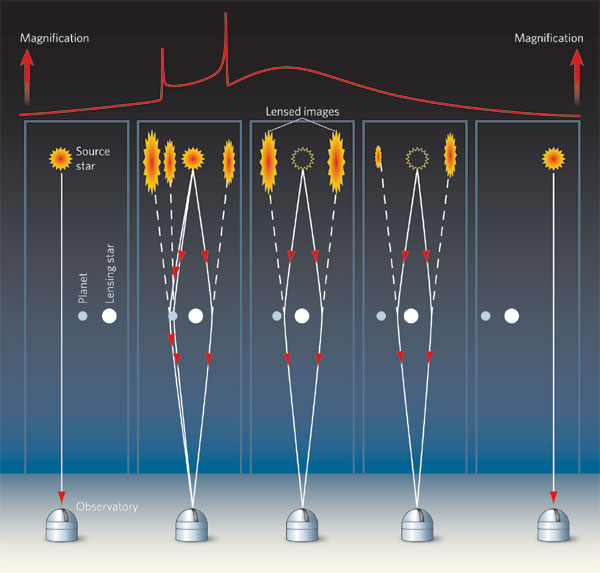
\includegraphics[width=.63\columnwidth]{figures/microlensing.jpg}
    \caption{Credits: Didier Queloz, \emph{Nature} \textbf{439}, 400--401.
      \doi{10.1038/439400a}}
    \vspace{-1em}
  \end{figure}
\end{frame}

\begin{frame}
  \frametitle{Binary Lens with Orbital Motion}
  In microlensing events, usually, static binary systems are taken into account,
  but binary systems do rotate

  The parameters to be determined using a fit in microlensing events by binary
  lens with orbital motion are
  \begin{itemize}
  \item base parameters: \(t_{0} \quad u_{0} \quad t_{\textup{E}} \quad \theta\)
  \item finite source effects: \(\rho_{\star}\)
  \item binary lens: \(b \quad q\)
  \item binary lens with orbital motion: \(a \quad e \quad i \quad \phi\)
  \end{itemize}
  In addition, with small mass ratios \(q\) there is the \alert{close-wide
    degeneracy} \(b \longleftrightarrow b^{-1}\)

  What if we knew the orbital period of the lenses
  \begin{equation*}
    P = 2\pi\sqrt{\frac{a^{3}}{G(m_{1} + m_{2})}} =
    2\pi\sqrt{\frac{a^{3}}{Gm_{1}(1 + q)}}
  \end{equation*}
  \alert{independently}?
\end{frame}

\begin{frame}
  \frametitle{Simulation}
  \begin{figure}
    \centering
    \vspace{-0.5em}
    \href{run:./movie.mp4}{
      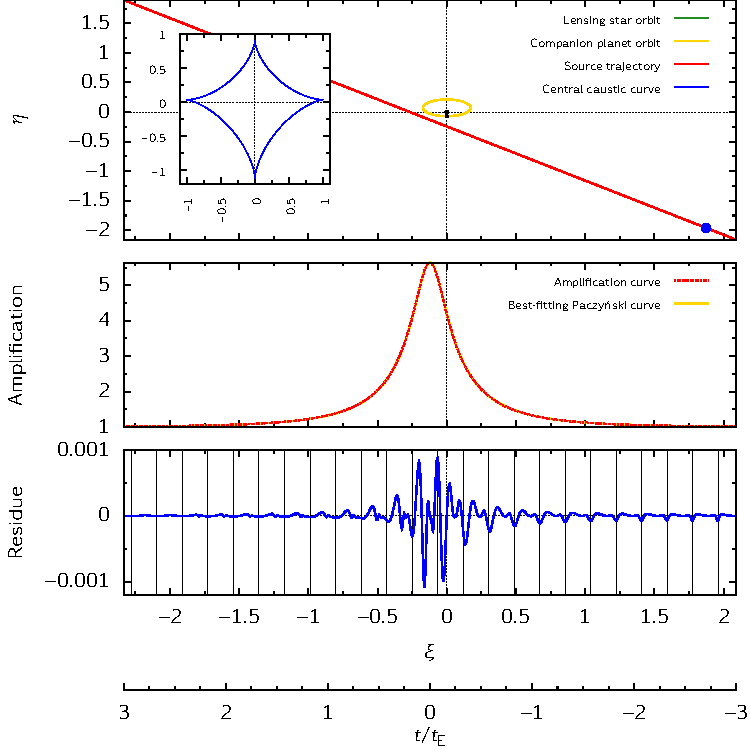
\includegraphics[width=0.6\columnwidth]{figures/figure2}}
    \caption{\(q = 10^{-3}\), \(a = 0.2\), \(e = 0.5\), \(i =
      \SI{45}{\degree}\), \(\phi = \SI{0}{\degree}\), \(P = t_{\textup{E}}/4\)}
    \vspace{-1.2em}
  \end{figure}
\end{frame}

\begin{frame}
  \frametitle{Simulation (periodogram)}
  \begin{figure}
    \centering
    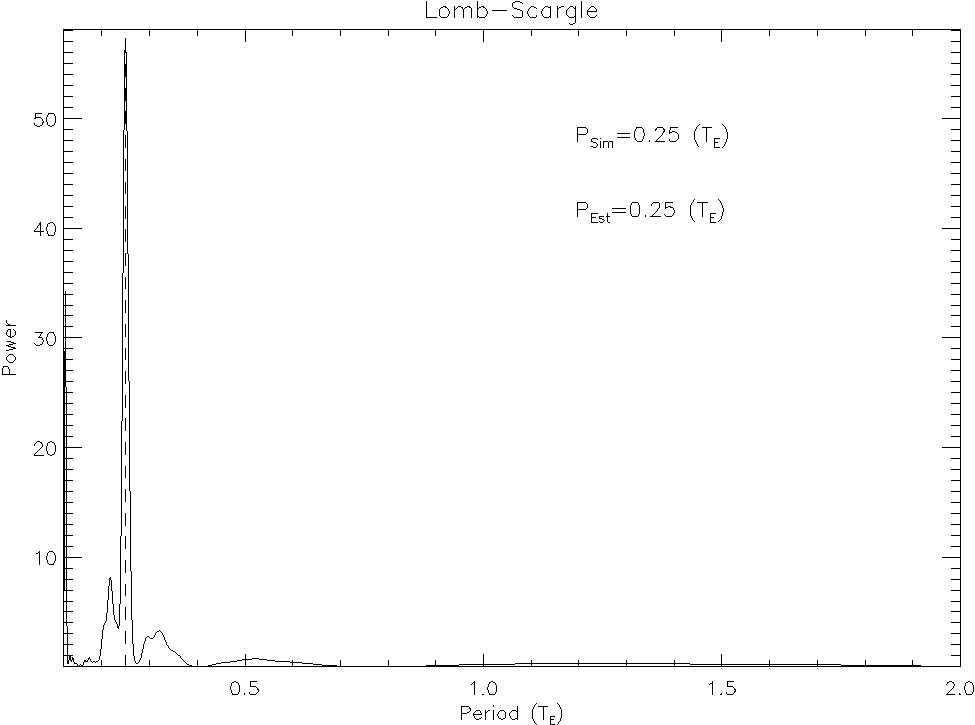
\includegraphics[width=0.85\columnwidth]{figures/lombscargle2}
  \end{figure}
\end{frame}

\begin{frame}
  \frametitle{Fit to Real Data}
  \begin{figure}
    \centering
    \vspace{-0.5em}
    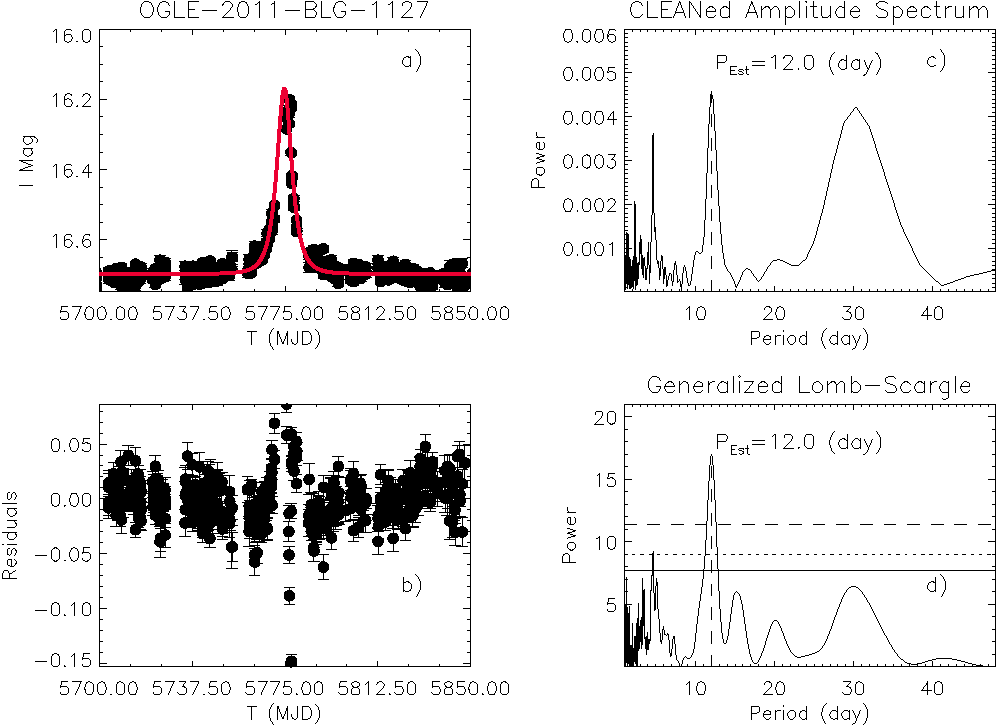
\includegraphics[width=0.77\textwidth]{figures/ogle322all}
    \caption{Event OGLE-2011-BLG-1127/MOA-2011-BLG-322}
    \vspace{-1.2em}
  \end{figure}
\end{frame}

\begin{frame}
  \frametitle{Conclusions}
  \begin{itemize}
  \item[\advice] Orbital period of the lenses should be \alert{shorter} than the
    Einstein time of the event or we must have a \alert{long observational
      window}
  \item[\advice] We fit the observed amplification curve to a \alert{simple
      Paczyński curve}, with four easily-guessable free parameters, and then
    perform a periodogram on the residue curve: the period so obtained is the
    \alert{period of the binary system}
  \item[\warning] We need to \alert{remove a very small region} around the
    maximum peak from the residue curve before performing the periodogram
  \item[\warning] Periodic feature with the same period far from the peak
    \(\implies\) \alert{source periodicity} (binary system, intrinsic variable,
    etc\dots)
  \end{itemize}
\end{frame}

\begin{frame}
  \frametitle{Reference}
  \nocite{*}
  \printbibliography{}
\end{frame}

\end{document}

%%% Local Variables:
%%% mode: latex
%%% TeX-master: t
%%% ispell-local-dictionary: "american"
%%% End:
